\chapter{引言}\label{chap:introduction}

\section{研究背景}

LGAD是在标准的硅探测器的$n^{++}$层下面增加一层$p^{+}$,形成$n^{++}$-$p^{+}$-$p$-$p^{++}$结构,
以此在结合处获得足够高的电场,其结构如图~\ref{fig:lgadstructure}所示。对于给定的$n^{++}$层,LGAD的增益受$p^{+}$的掺杂和结构的影响。
当带电粒子穿过探测器时,载流子(电子空穴对)的漂移会引起初始电流的产生,随后电子到达增益层,新的电子空穴对产生,
空穴继续向LGAD底部漂移,电流增大。这个过程中的电荷增益就是LGAD的增益,LGAD的输出信号与LGAD的增益大小成正比。
时间分辨中jitter的贡献,既受$dV/dt$大小的影响,又受探测器电容的影响,综合考虑最终决定了采取$50\ \mu \rm m$有效厚度的设计方案,
LGAD总厚度$300\ \mu \rm m$(包含support wafer的厚度)。

\begin{figure}[!htbp]
    \centering
    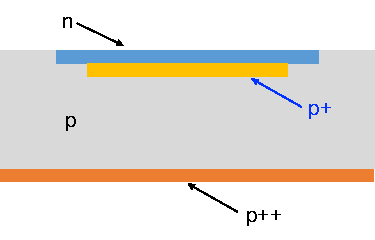
\includegraphics[width=0.40\textwidth]{lgadstructure}
    \bicaption{LGAD的结构示意图}{Structure diagram of LGAD}
    \label{fig:lgadstructure}
\end{figure}

日本滨松(Hamamatsu Photonics)设计并流片了HPK single LGAD,如图~\ref{fig:hpklgad},有效区域为$1.3\times 1.3\rm \ mm^{2}$,总尺寸$2.3\times 2.3\rm \ mm^{2}$,
中心圆形pad用于信号收集,周围有8个guard ring接口。

\begin{figure}[!htbp]
    \centering
    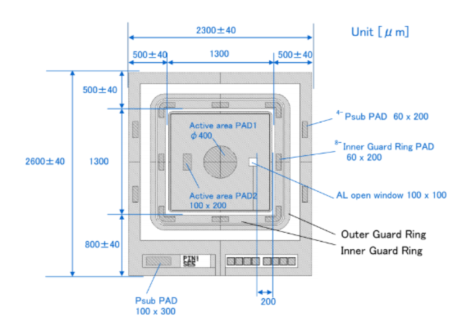
\includegraphics[width=0.70\textwidth]{hpklgad}
    \bicaption{HPK LGAD设计图}{Designed diagram of HPK LGAD}
    \label{fig:hpklgad}
\end{figure}

瞬态电流技术TCT是一种确定硅探测器电场分布的方法。利用电离辐射或激光在反向偏压探测器内产生的电子空穴对的漂移和扩散。
在电场影响下,载流子漂移并在读出电极中产生电流。电流脉冲包含有关漂移电荷量及其迁移速率的信息。根据光照方向,
TCT可分为top-TCT(简称TCT)和edge-TCT两种技术。我们用红外激光器研究了HPK LGAD的电场分布,原理图如图~\ref{fig:tctschematic}所示。
波长为$1024\rm \ nm$的红外激光在LGAD侧面聚焦进行纵向扫描,并且给示波器提供触发信号,xyz table用于调整LGAD的位置与到激光器之间的距离。
Keithley 2410给LGAD提供外部电场,LGAD由此产生的信号经过放大器由示波器采集并记录。

\begin{figure}[!htbp]
    \centering
    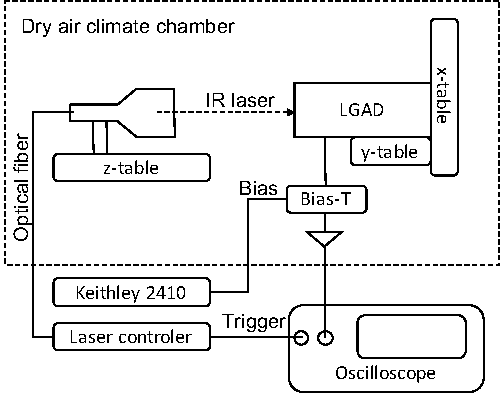
\includegraphics[width=0.70\textwidth]{tctschematic}
    \bicaption{TCT工作原理图}{Schematic diagram of TCT}
    \label{fig:tctschematic}
\end{figure}

此LGAD的耗尽电压约为$48\rm \ V$,截断电压约为$250\rm \ V$。我们选取了$40\rm \ V$、$50\rm \ V$、$100\rm \ V$、$150\rm \ V$、$200\rm \ V$进行了扫描。低于耗尽电压时(如$40\rm \ V$),
输出信号不明显,高于耗尽电压时(如$50\rm \ V$),开始出现输出信号。随着外部电压的增大,输出信号有了明显的增强,
但信号收集时间基本在$3\rm \ ns$内结束(电压高于耗尽电压时,如图~\ref{fig:hpklgad_tct_waveform})。随着电压的提高,LGAD的信号也有了明显的提升。
在信号产生的瞬间,我们可以认为载流子只受到电场力的作用,且载流子初始速度近似为$0$,在刚开始运动的时刻可近似看作加速度恒定的加速运动,
qE=mv/t,则v=qEt/m,载流子的迁移速率与此处的电场大小成正比。信号上升的上升沿($0-1\rm \ ns$)近似为一次函数,积分面积与信号的大小成正比,
因此载流子的迁移速率与信号积分面积成正比。我们取$0-0.5\rm \ ns$之间信号对时间的积分来表征LGAD内载流子迁移速率的相对大小,如图~\ref{fig:hpklgad_tct_velocity}所示。
横坐标$0\rm \ mm$处为LGAD顶部,$0.05\rm \ mm$处为LGAD底部。我们可以看到在接近LGAD顶部区域的电场比bulk区高很多,
并且随外加电场的提高载流子的迁移速率也有明显的加快,即使接近截断电压,迁移速率也不会饱和。
在靠近LGAD底部出现了另外一个电场增强的小峰,来自于LGAD bulk区和$p^{++}$层中空穴密度差异。
此外,我们还对收集电荷做了估计,用来计算LGAD的增益大小。为保证信号结束,我们对信号开始后$20\rm \ ns$的电压进行积分,
计算出电荷的相对大小见图~\ref{fig:hpklgad_tct_charge}。

\begin{figure}[!htbp]
    \centering
    \begin{subfigure}[b]{0.3\textwidth}
      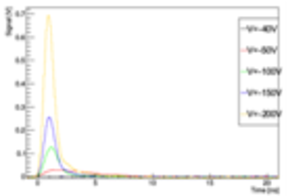
\includegraphics[width=\textwidth]{hpklgad_tct_waveform}
      \caption{}
      \label{fig:hpklgad_tct_waveform}
    \end{subfigure}
    ~
    \begin{subfigure}[b]{0.3\textwidth}
      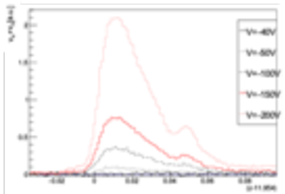
\includegraphics[width=\textwidth]{hpklgad_tct_velocity}
      \caption{}
      \label{fig:hpklgad_tct_velocity}
    \end{subfigure}
    ~
    \begin{subfigure}[b]{0.3\textwidth}
      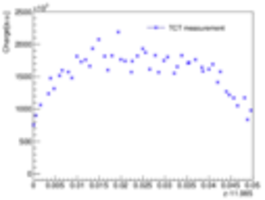
\includegraphics[width=\textwidth]{hpklgad_tct_charge}
      \caption{}
      \label{fig:hpklgad_tct_charge}
    \end{subfigure}
    \bicaption{ Edge-TCT测试结果:(a) 不同电压下,LGAD增益层信号;
    (b) 一定电压下,LGAD内部纵向载流子迁移速率相对大小分布,$0\rm \ mm$处为LGAD顶部,$0.05\rm \ mm$处为LGAD底部;
    (c) $200\rm \ V$电压时,LGAD收集电荷相对大小分布。}
    { Results from edge-TCT measurement: (a) Wavefrom from LGAD at different bias voltages; 
    (b) Relative velocity of carriers inside LGAD at certain bias voltages, LGAD top at $0\rm \ mm$ and LGAD bottom at $0.05\rm \ mm$; 
    (c) Relative charge collection from LGAD at bias voltage of $200\rm \ V$.}
    \label{fig:hpklgad_tct}
\end{figure}
























\section{系统要求}\label{sec:system}

\href{https://github.com/mohuangrui/ucasthesis}{\texttt{ucasthesis}} 宏包可以在目前主流的 \href{https://en.wikibooks.org/wiki/LaTeX/Introduction}{\LaTeX{}} 编译系统中使用,如\TeX{}Live和MiK\TeX{}。因C\TeX{}套装已停止维护,\textbf{不再建议使用} (请勿混淆C\TeX{}套装与ctex宏包。C\TeX{}套装是集成了许多\LaTeX{}组件的\LaTeX{}编译系统。 \href{https://ctan.org/pkg/ctex?lang=en}{ctex} 宏包如同ucasthesis,是\LaTeX{}命令集,其维护状态活跃,并被主流的\LaTeX{}编译系统默认集成,是几乎所有\LaTeX{}中文文档的核心架构)。推荐的 \href{https://en.wikibooks.org/wiki/LaTeX/Installation}{\LaTeX{}编译系统} 和 \href{https://en.wikibooks.org/wiki/LaTeX/Installation}{\LaTeX{}文本编辑器} 为
\begin{center}
    %\footnotesize% fontsize
    %\setlength{\tabcolsep}{4pt}% column separation
    %\renewcommand{\arraystretch}{1.5}% row space 
    \begin{tabular}{lcc}
        \hline
        %\multicolumn{num_of_cols_to_merge}{alignment}{contents} \\
        %\cline{i-j}% partial hline from column i to column j
        操作系统 & \LaTeX{}编译系统 & \LaTeX{}文本编辑器\\
        \hline
        Linux & \href{https://www.tug.org/texlive/acquire-netinstall.html}{\TeX{}Live Full} & \href{http://www.xm1math.net/texmaker/}{Texmaker} 或 Vim\\
        MacOS & \href{https://www.tug.org/mactex/}{Mac\TeX{} Full} & \href{http://www.xm1math.net/texmaker/}{Texmaker} 或 Texshop\\
        Windows & \href{https://www.tug.org/texlive/acquire-netinstall.html}{\TeX{}Live Full} 或 \href{https://miktex.org/download}{MiK\TeX{}} & \href{http://www.xm1math.net/texmaker/}{Texmaker}\\
        \hline
    \end{tabular}
\end{center}

\LaTeX{}编译系统,如\TeX{}Live(Mac\TeX{}为针对MacOS的\TeX{}Live),用于提供编译环境,\LaTeX{}文本编辑器 (如Texmaker) 用于编辑\TeX{}源文件。请从各软件官网下载安装程序,勿使用不明程序源。\textbf{\LaTeX{}编译系统和\LaTeX{}编辑器分别安装成功后,即完成了\LaTeX{}的系统配置},无需其他手动干预和配置。若系统原带有旧版的\LaTeX{}编译系统并想安装新版,请\textbf{先卸载干净旧版再安装新版}。

\section{问题反馈}

请见 \href{https://github.com/mohuangrui/ucasthesis/wiki/%E5%B8%B8%E8%A7%81%E9%97%AE%E9%A2%98}{问题反馈} 

欢迎大家有效地反馈模板不足之处,一起不断改进模板。希望大家向同事积极推广\LaTeX{},一起更高效地做科研。

\section{模板下载}

\begin{center}
    \href{https://github.com/mohuangrui/ucasthesis}{Github/ucasthesis}: \url{https://github.com/mohuangrui/ucasthesis}
\end{center}
